\chapter{多铁材料的应用与发展前景}

\section{多铁材料的应用}
多铁材料在各个领域都有着及其重大的应用前景,尤其是在信息存储领域。利用多铁材料铁电铁磁耦合的性质可以制作“磁读电写”存储器,实现高可靠性、低能耗、高速度存储。

% \begin{itemize}
%     \item 多态存储器
    
%     多铁材料同时拥有铁磁性与铁电性两种性质,用这两种性质的四种组合可以存储数据,存储密度比传统的磁存储存储密度有着巨大的提高。

    
%     \item 低能耗逻辑存储器
%     \item 磁电探测器
%     \item 高频射频器件
    
% \end{itemize}
\paragraph{多态存储器}
多铁材料同时拥有铁磁性与铁电性两种性质,用这两种性质的四种组合可以存储数据,存储密度比传统的磁存储存储密度有着巨大的提高。
与传统的磁存储与电存储相比具有两种铁性质的多铁材料无疑在信息存储技术方面会占有巨大的优势。通过外加电磁场的调控,可以实现四种阻值的状态,通过合适的工业技术手段,可以实现对存储效率的倍增。

\paragraph{低能耗逻辑存储器}
目前寻求更高效的低能耗存储器是计算机技术的一个重要的发展方向。现在的发展趋势是将自旋霍尔效应与多铁材料的电场调控磁性相结合,制成多铁性的包含强自旋轨道耦合的逻辑存储器。通过自旋霍尔效应可以将自旋转化为电荷或者电场,而多铁性的铁电铁磁耦合可以利用电场调控磁性或自旋,如果这样的存储器可以研制成功,器件整体工作电压将从5V左右降低到100mV,反转或存储一比特信息所需要的能量将有希望降低到1aJ。就目前来说,在众多发现的材料之中,最古老的多铁材料$BiFeO_{3}$希望最大。




\paragraph{高频射频器件}
高频射频器件也是多铁材料的重要应用方向之一。高频射频器件在无线通信、国防军事等方面有着重大应用价值,就目前研究来看,此方向应用最多的是基于机械耦合的多铁材料。

\paragraph{磁电探测器}
多铁性材料最直接的应用之一就是磁电传感器,多铁材料内部铁电性与铁磁性相耦合的性质可以很容易地实现电信号与磁信号的相互转化。相对于传统的磁电传感器,基于多铁材料电磁耦合效应的磁电探测器在工作时不需要消耗能量,可以做成无源器件,对简化电子电路有很大价值。
\begin{figure}[h]
    \centering
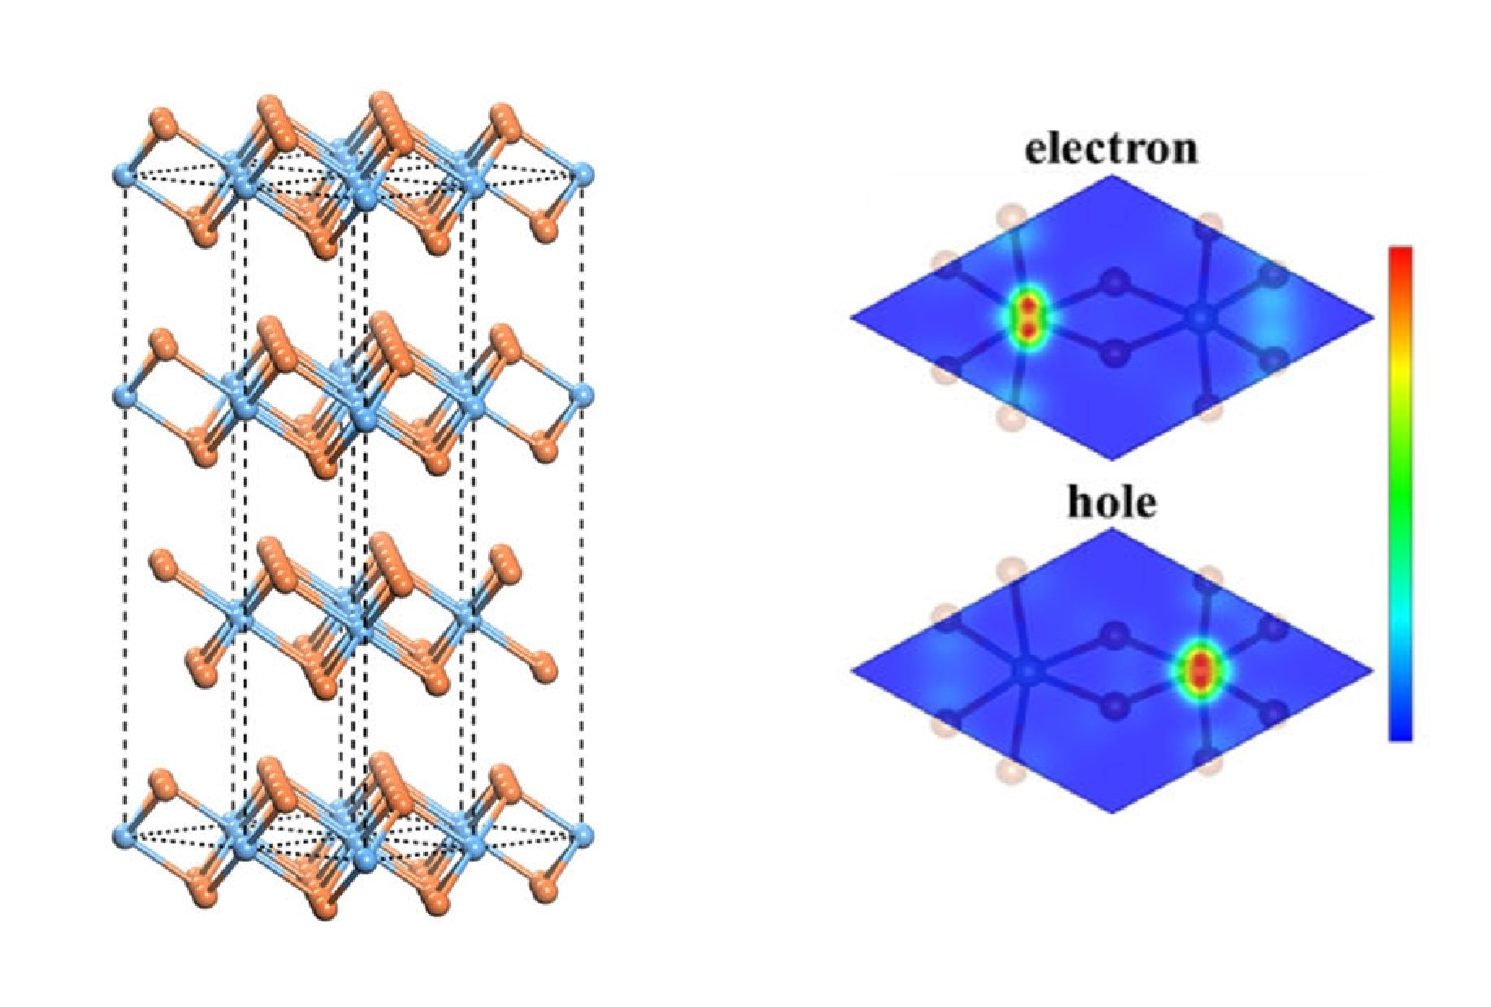
\includegraphics[width=0.8\textwidth]{./pic/010-4.png}
\caption{层状溴化铬结构与溴化铬掺杂电子或空穴后的电子密度分布变化。}

\label{dog010-4}
\end{figure}


\subsection{多体材料研究的展望}

有待解决的若干重大问题与相关要点:
\begin{itemize}
    \item 发现一种室温强耦合的新型多铁材料\\
目前发现的多铁材料都有或多或少的缺点,距离现实实际的生产生活仍然有着一定的距离。为了达到应用的目的,仍然需要寻找出室温下稳定性高,电磁性质关联度高的多铁材料。寻找能广泛应用的多铁材料是贯穿整个多铁材料研究的重要目的之一。
    \item 利用原子尺度设计与逐层生长技术相结合,改良现有的多铁复合材料\\
随着新的实验与理论工具的不断成熟与发展,原子尺度设计与逐层生长技术成为制备寻找新型使用多铁材料的重要手段之一。
    \item 发展并提出新的电磁耦合机制,探索与接近理论极限 \\
从当今对多铁材料的研究看来,还是没有一种完美的对多铁性质的通用解释。随着人们对多铁材料的实验积累越来越多,对多铁材料的认识越来越深入,需要新的更合适的理论方案来解释新的实验现象与对新材料进行理论计算预测。
    \item 理解控制与应用铁磁铁电转换动力学\\
多铁材料研究的核心之一是多铁材料内部铁磁性与铁电性的耦合关系与具体实现机制,磁相互作用与电相互作用的转换动力学是研究的关键点之一。
    \item 多铁性在物理学其他领域的现象与作用\\
多铁性材料在凝聚态物理的其他领域或许有着其他新现象或者作用。
\end{itemize}

\begin{figure}[h]
    \centering
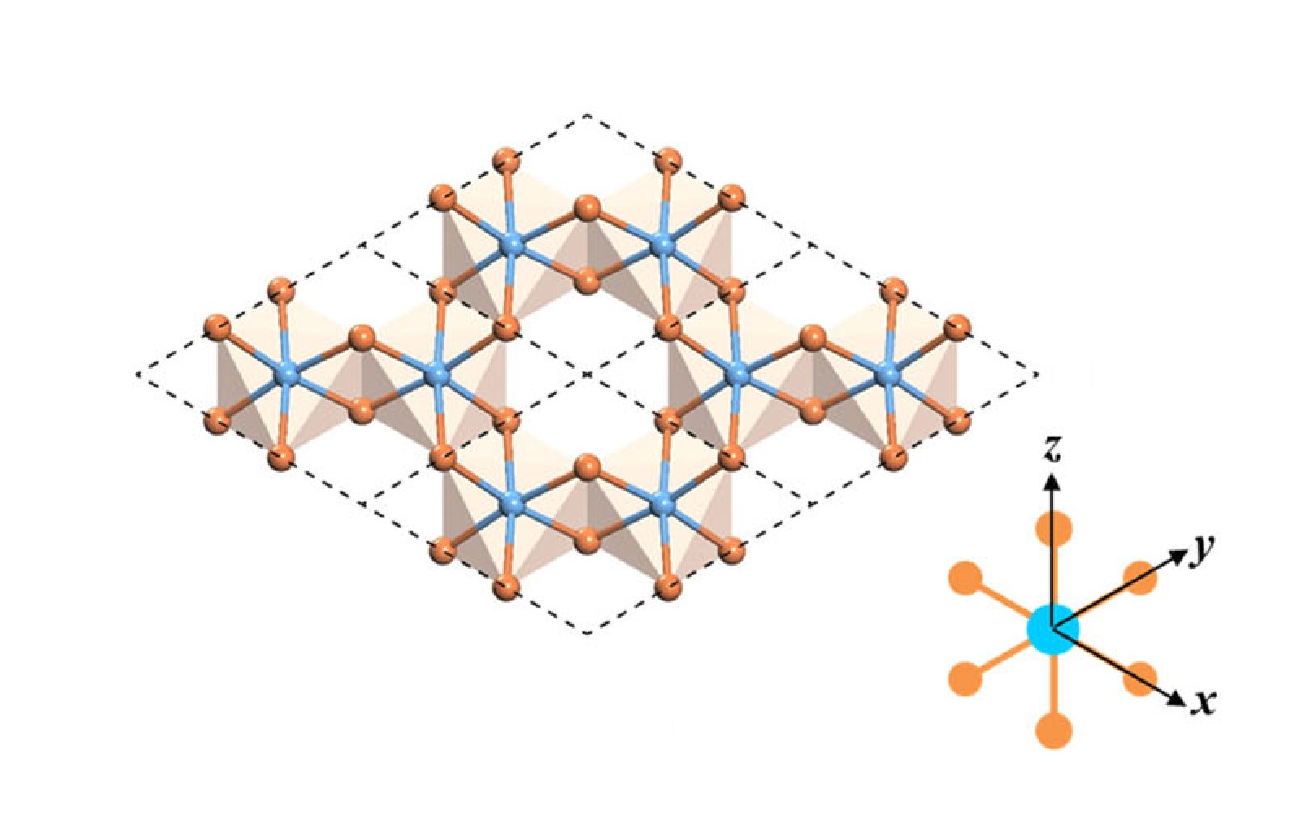
\includegraphics[width=0.8\textwidth]{./pic/010-2.png}
\caption{二维溴化铬微观结构\ 每个铬离子与周围六个溴离子相连,一个溴离子与两个铬离子相连。铬离子在空间平面中构成六边形网状结构。}

\label{dog010-2}
\end{figure}

\section{材料理论计算的新方法与发展}

\subsection{高通量计算材料学}

随着先进的自动化计算技术的进一步完善与发展,通过计算预测、发现、设计新材料的准确度、可靠性、计算效率进一步提高,近年来,随着机器学习等计算机技术的发展,利用数据挖掘进行高通量筛选新材料研究越来越受到重视。以二维材料为例,利用自动化工具可以在已知的材料里面筛选出二维材料。进行数据材料筛选,首先需要有一个筛选范围,通常是完备的晶体学数据库。由于二维材料等低维材料层状结构之间存在着巨大的空隙,其原子的共价体积与晶格原包的体积之比比较小,首先将填充比在0.15~0.50筛选出来。然后再筛选层状结构的层间距离较大的材料,最后在检查层状结构之间有没有共价键穿过。这种筛选方法固然会漏掉一些材料,但可以筛选出大部分的二维材料。

\subsection{演化算法}

随着现代计算机技术的发展与进步,理论计算在发现新材料的过程之中起着越来越重要的作用。在计算机科学落后的过去,计算能力的有限限制了采用大规模计算的方式进行材料筛选的方式,只能在实验上采取试错法等低效率的方法进行,在这个过程之中,新材料的能否发现与发现过程是否顺利在客观实验条件之外主要取决于实验参与人员的经验与熟练程度。到了计算技术成熟发展的今天,利用理论计算工具对材料进行初步筛选大大加快了新型材料的发现与实验成功率。

利用计算机技术对众多材料结构进行预测的核心问题是找到以众多参数为因变量的目标性质参数函数的全局最小值,由于材料类型多种多样,结构种类各异,组成元素千奇百怪,对所用的可能的元素组合与结构变化全部计算一次是显然不可能的,必须利用一些特殊的技巧对计算过程进行简化。目前已经存在多种有效方法进行结构预测,主要有:遗传算法、随机取样、微分演化算法、模拟退火等方法。其中演化算法是一种比较有代表性的算法,可以分为五个步骤:产生初始结构、结构弛豫、相似性分析与适应度函数、产生新结构、收敛性判断等五个步骤。

\subsubsection{初始结构}

初始结构是演化算法预测新材料的第一步,为了减少不必要的计算通常应该从晶格结构的对称性方面考虑并对原子位置加以限制,对于二维结构来说,分别对应17个平面群与80个层空间群。一旦一个原子的位置确定之后,其对称性位置可以通过空间群的点群矩阵和平移矢量得到:
\begin{equation}
    \begin{split}
        \tilde{ x}_{1}= W_{11}x_{1}+W_{12}x_{2}+W_{13}x_{3}+\bm{w}_{1} \\
        \tilde{ x}_{2}= W_{21}x_{1}+W_{22}x_{2}+W_{23}x_{3}+\bm{w}_{2} \\
        \tilde{ x}_{3}= W_{31}x_{1}+W_{32}x_{2}+W_{33}x_{3}+\bm{w}_{3} \\
    \end{split}
    \label{eq:jg}
\end{equation}
在通过点群的周期性结构平移之后,还需要加上若干硬性的限制,以使得所构造的结构符合物理事实,包括不限于以下限制:原子间的最小距离、在给定原子数目下晶格的大小等。具体的限制要结合所研究的条件尺度体系等具体设置。

\subsubsection{结构弛豫}

几何结构弛豫在第一性原理计算方面已经发展成熟,各种软件都有着成熟的体系来进行结构弛豫,通常采用的方法有最速下降法、准牛顿法、共轭梯度法等相关方法。进行结构弛豫之后不仅可以优化结构及其能量,还可以得到结构的一些其他性质,并且可以为下一步的结构相似性分析提供数据支撑与前提条件。

\subsubsection{相似度分析与适应度函数}

在结构弛豫之后,会有大量的大量结构优化到统一构型,如果不加以甄别会造成大量的重复计算,从而降低结构的多样性与寻找新结构的效率。为了解决这一问题,需要进行相似度分析,通过定义相关结构的数学特征量可以定量导出两种结构的相似度,通过对高相似度结构的合并与归类,可以大大减少不必要的计算。比较常用的一个原子键加权平均指标为:
\begin{equation}
    \bar{Q}_{lm}^{\delta_{AB}}=\frac{1}{N_{AB}}\sum_{i \in A,j \in B}e^{-\alpha(r_{ij}-b_{AB})}Y_{lm}(\theta_{ij},\phi_{ij} )
    \label{eq:jjq}
\end{equation}

其中$Y_{lm}(\theta_{ij},\phi_{ij} )$是球谐函数,与两个原子之间的相对位置有关,$\theta_{ij}\text{和}\phi_{ij}$是化学键的方位角,$\delta_{AB}\text{和}N_{AB}$分别是键的类型与数目。考虑上参考系变换的不变性,可以对m进行求和:
\begin{equation}
    Q_{l}^{\delta_{AB}}=\sqrt{\frac{4\pi}{2l+1}\sum_{m=-l}^{l}|\bar{Q}_{lm}^{\delta_{AB}}|^{2}}
    \label{eq:jjq2}
\end{equation}
这样就可以得到不同键的特征值,最终组成键结构的特征矩阵,利用这一矩阵可以定义两种结构之间的差异:
\begin{equation}
    D_{UV}=\sqrt{\frac{1}{N_{type}}\sum_{\delta_{AB}}\sum_{l}(Q_{l}^{\delta_{AB},U}-Q_{l}^{\delta_{AB},V})^{2}}
    \label{eq:jjq3}
\end{equation}

通过相似性筛选之后,需要对这些不同的结构进行筛选,选出“好”结构,一般是选择能量最低,比较稳定的结构,如果对材料的某种功能进行逆向设计,则需要采用其他的标准进行分类评判。

\subsubsection{产生新结构}

利用原有的结构经过一系列的操作产生新的结构,是演化算法的一大特点。产生新结构的首要问题就是选取那些老结构作为新结构产生的依据。截断法是一个比较经常采用的方法,取某种指标的一个定值作为标准,只选取达标的部分。组合法划分为多个小组,在各个小组内部分别选择。随机法是在指标的基础上加上随机数的影响。以上的方法也可以混合使用,随机数的引入可以增强结构的多样性。产生新结构的方法也有很多种常见的有遗传算法、粒子群优化算法和微分演化算法等方法。

\paragraph{遗传算法}遗传算法一般采用混合和变异来产生新的结构。以二维材料为例,在若干结构内部划分为多个部分,在不同结构中随机选取并交换一部分,在进行必要的调整之后可以作为新的结构供应下一代使用。变异方法是大范围引入随机性,可以随机改变原子位置,随机改变原子种类,随机改变晶格结构。以二维材料为例,可以通过下面的变换矩阵进行随机微调:
\begin{equation}
    [\bm{I}+\epsilon_{ij}]=
    \begin{pmatrix}
        1+\epsilon_{11}&\frac{\epsilon_{12}}{2}&0\\
        \frac{\epsilon_{12}}{2}&1+\epsilon_{22}&0\\
        0&0&1
    \end{pmatrix}
    \label{eq:yc}
\end{equation}
其中$\epsilon$是随机数。随机数的引入有助于保持结构的多样性,对搜索低能结构附近的势能面非常重要。

\paragraph{粒子群优化算法}粒子群优化算法来源于仿生学,主要受到自然界的群体生物的群体活动智能系统的启发。在某些自然界的生物组群之中存在着广泛的自组织行为。在众多仿生学算法之中,粒子群优化算法是其中一个重要的算法。
\paragraph{微分演化算法}
微分演化算法的核心是考虑不同之间差别,其通用表达式为:
\begin{equation}
    p'_{i}=\gamma p_{best} +(1-\gamma)p_{i}+F(p_{r1}-p_{r2})
    \label{eq:sf}
\end{equation}
其中$p_{r1}\text{和}p_{r2}$是母代之中随机选取的两个个体,针对具体问题的操作还是要结合实际情况考虑。

\subsubsection{收敛性判断}

判断结果是否收敛是整个计算过程的最后一步,根据遗传算法的原理,计算可以无穷无极迭代下去,但这显然是没必要且不可能的,为了尽可能减少计算量与得到结果,通常需要设定一个收敛判据。判断方法有很多种,最直接的一种是如果计算多代之后效果没有明显提高,即可认为结果已收敛,可以结束计算了。

\subsection{机器学习}

随着现代计算机技术的发展与进步,以薛定谔方程与密度泛函理论为基础的计算方法在凝聚态物理、材料科学与计算化学中发挥着越来越重要的作用。计算机技术这一重要工具与手段对基础学科的发展有着巨大的促进作用。在二十一世纪,机器学习这一新兴的计算机技术开始在各个领域发挥作用,将机器学习等人工智能技术与手段在计算材料领域也有着巨大的应用前景。机器学习与人工智能技术作为一种新兴手段在很多领域可以取代人类做一些重复性的工作,越来越多领域开始采用这种方法来进行辅助工作,随着机器学习应用范围越来越广,机器学习技术应用的资源和工具意味着进入的障碍比以往任何时候都要低。

\begin{figure}[h]
    \centering
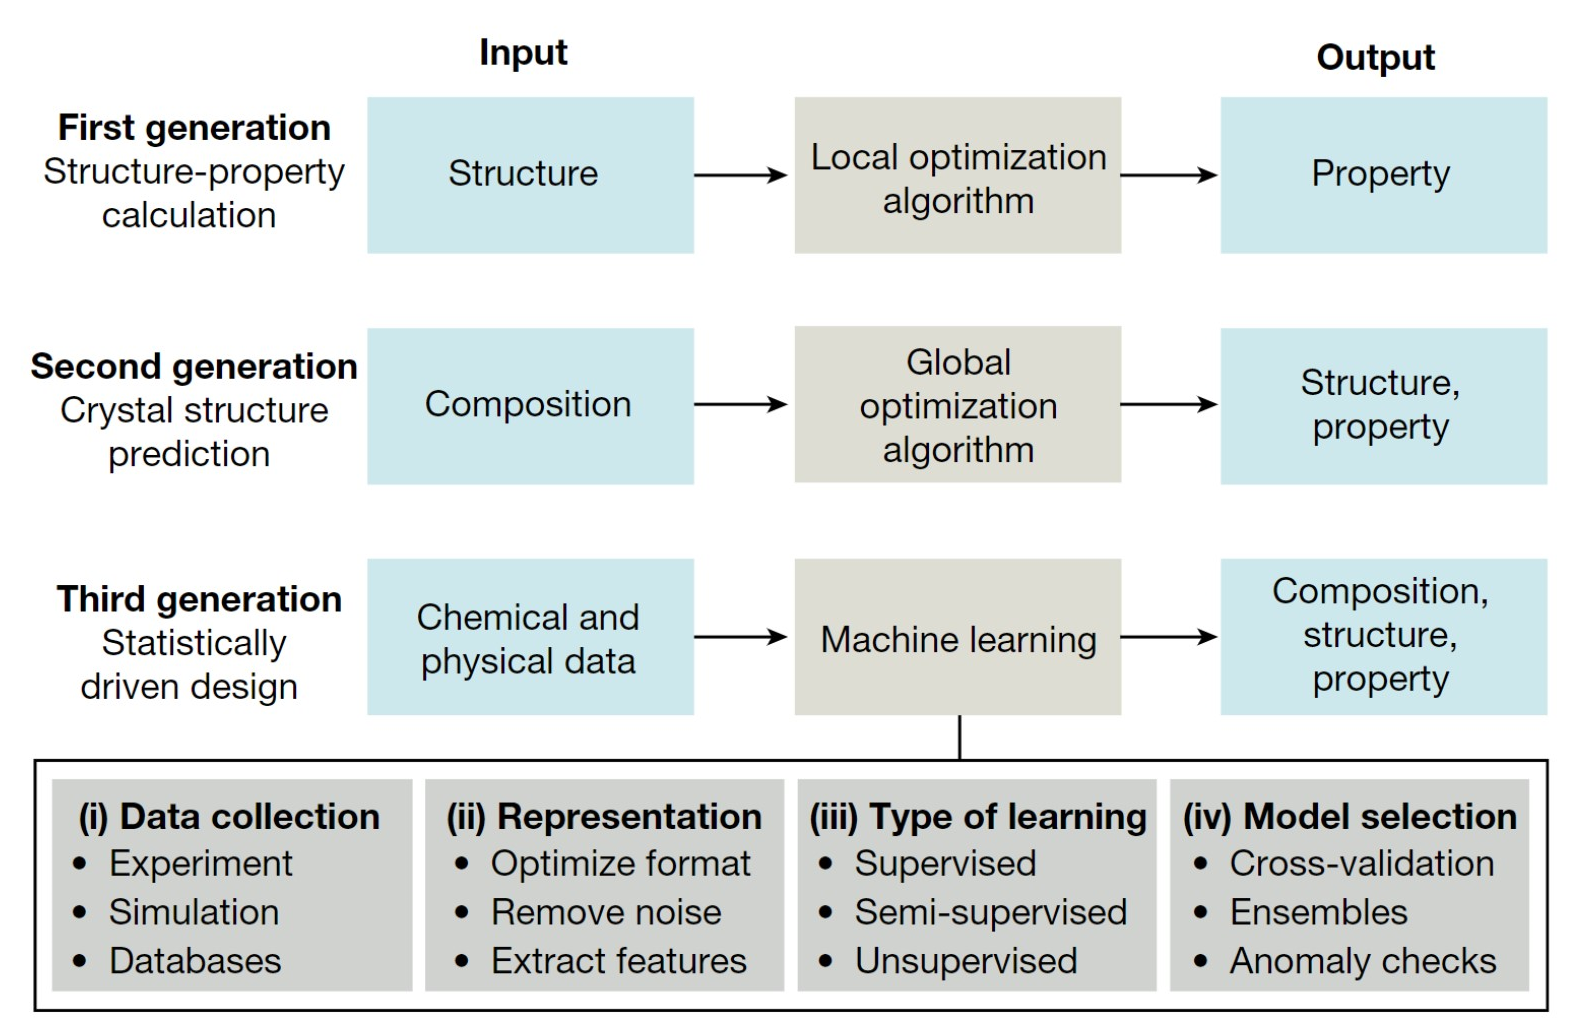
\includegraphics[width=0.8\textwidth]{./pic/025.png}
\caption{计算材料学的三代方法 \ 第一代方法是输入物质的物理结构,通过第一性原理计算等方式导出物质的性质,并通过结构与性质的对应关系来实现新材料的发现与设计。第二代采用全部据优化方法,输入物质的组成,通过一系列算法输出结构与性质。第三代是通过机器学习,输入基础的物理化学规则与数据,全自动地输出材料的组分结构与性质。机器学习的方法自动化程度更高,但是其计算过程难以理解与解释。}

\label{dog025}
\end{figure}

机器学习等方法并不是万能的,相关的模型参数等也不会凭空产生,机器学习的方法需要足够多的数据。只要有足够多的数据与合适的规则发现算法,计算机就可以确定已知的或者尚未发现的规律。与传统计算方式相比,机器学习方法主要通过学习数据的一部分并自动化建立模型来拟合数据的另一部分,通过优化后的模型来辅助解决实际问题。

\subsubsection{机器学习在计算材料学应用的一般方法}

\paragraph{收集数据}
数据是机器学习的核心之一,是决定工作成败的一个重要因素。数据不会凭空产生,足够多的准确数据是机器学习的前提条件。虽然现在有很多晶体学数据库,但并不能直接拿来作为数据源,需要结合实际问题从数据库中挑选出合适的数据。

所需要数据的类型结构与数量与所选取的学习方法也有关系,通常的学习方法有监督学习、半监督学习与无监督学习。有监督学习包含输入与输出,目的是根据输入数据产生一个具有相当可信度的输出预测值,这类数据需要输入与正确的预测值。无监督学习通常不需要进行输出,一般用来进行识别数据中的趋势、模式与聚类。半监督学习主要应用在输入数据远多于输出数据的情况下,通常可作为数据生成器使用。

\paragraph{数据预处理}
找到正确合适的数据集之后并不能直接拿来用,需要对数据进行预处理,对数据中的错误与噪声等对下一步造成障碍的不利因素要剔除出去。从各种途径采集到的原始数据并不一定总可以适应算法,适当对数据进行预处理,将数据从一种形式转化为另一种更合适的形式可能大大加快机器学习的进程。

理论上看来,数据与算法适应程度越高,进行机器学习的效果会越好,但实际上人们很难明确给出最适合的数据形式,只能猜测出一个大概符合的数据形式。在研究分子问题时,库伦矩阵可以很好概括原子核周围的势能信息,而且在平移与旋转分子时也是不变的。在周期结构中,由于晶格对称性与周期性,传统平移向量与分数坐标等方法并不总是合适,因为可以通过选择不同的坐标系以无数种方式表示晶格。在表示周期性结构的晶格时通常采用径向分布函数等方法。

\paragraph{选择算法}

选择完成合适的数据集之后,下一步就是选择合适的算法,就像数据预处理的方式要与算法相适应一样,数据集也应该与算法相适应。有些问题比如分类等,需要分立值输出,所选取的经过预处理之后的数据集也应该是不连续的,对于另一些问题,例如预测性质,所输出的是连续值,所采用的数据集也应该是连续的。在处理复杂问题时,单一的学习算法效果不一定好,有时候则需要将多种学习方式融合起来,组成更复杂的学习组合。常见的算法有:贝叶斯分类器、k近邻法、决策树方法、支持向量机。人工神经网络等方法。其中目前最为流行的是人工神经网络方法,这种方法是一种仿生学方法,起源是对大脑功能与结构的简单模仿。其数据处理功能的人工神经元可以分为输入层、输出层和隐藏层。神经元接受其他神经元传递的信息,经过简单计算之后传递给其他神经元。神经元之间的连接权重存储着整个网络学习到的知识,神经网络学习训练的过程实际上是调整优化权重的过程,这个过程类似于回归拟合预测,通过调整各个参数使得输出最优结果。

\paragraph{模型优化}
在选定合适的算法之后,还需要在计算过程之中进行微调,以使得所建立的模型更加接近真实情况。在进行机器学习的过程之中,经常会出现一些偏差,这些误差主要来源有三种,模型偏差、模型方差与不可约误差。模型偏差主要是由于模型自身问题造成的,模型与真实的物理过程存在着系统性的偏差。模型方差是指对输入数据的微小变动引起输出数据的剧烈波动。不可约误差通常是指由于训练数据中的噪声,测量限制,计算不确定性,或者仅仅是离群值或数据丢失而导致错误。通过对计算过程的适当调整可以减小模型偏差与模型方差。

模型偏差过大通常发生在模型复杂度不足以描述输入与输出值关系或者数据不足以支撑发现输入与输出之间的关系,而方差过大则发生在模型过于复杂,在处理输入输出关系时无中生有地臆造出并不存在的规则,这种情况通常叫做过拟合,其标志之一是在训练数据中正确率不断提高,而在测试数据中准确率不再提升或开始下降。在具体的操作过程之中应避免这种情况,可以用多组数据进行交叉验证来避免错误。

\begin{figure}[h]
    \centering
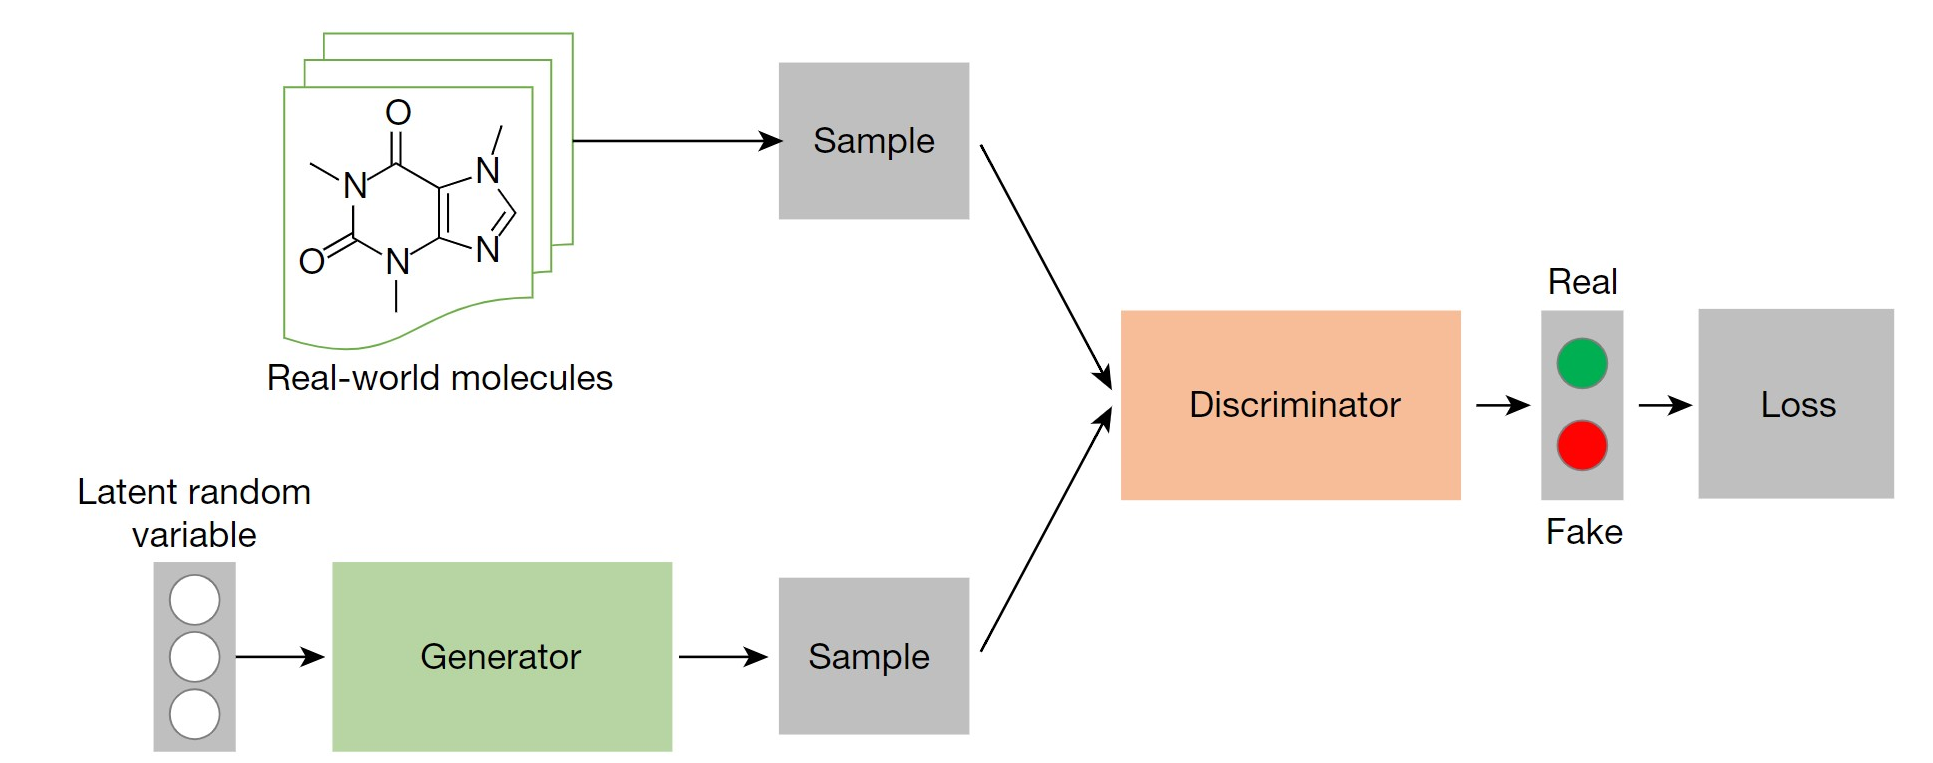
\includegraphics[width=0.8\textwidth]{./pic/026.png}
\caption{一种基于对抗生成网络的分子设计方法 \ 该方法是由两个网络做成的,一个生成器网络将随机数噪声转化为分子组合与结构,另一个判别器网络是将生成器网络造出来的分子结构与数据集中已知结构区分开,生成器的目的是使得所产生的分子结构不被判别器挑出来,而判别器的目的是选择出生成器产生的分子结构,两个网络相互对抗,协同学习,最终会使得输出结果接近真实的分子结构}

\label{dog024}
\end{figure}

\subsubsection{机器学习应用}

在材料领域,无论是理论计算还是实验领域,机器学习有着广泛的应用前景。机器学习可以用在指导化学合成,化学合成是一种很复杂的综合性问题,其应用型背景需要考虑成本、安全性、产率反应速率等多种因素。通过对文献中有机化学分子合成路线的学习,基于多层人工神经网络的深度学习方法设计出的有机物合成路线可以达到与人工专家无法区分的程度,但这种基于既有数据库的机器学习方法无法产生出超过已有知识体系的结果,即只能替代一些重复性的工作,无法进行创新性的工作。机器学习可也已进行一些数据辅助分析工作,在实验方面,应用不同的手段如X射线、中子衍射、核磁共振等对物质的结构与性质进行解析时会得到各有侧重的数据,每种方法都有其优点与局限性,机器学习方法可以用来发现多组数据之间的关联性。
% 通过对人工神经网络的学习与训练,还可以识别出物质相变时的过度
在计算大规模复杂系统时,机器学习可以代替DFT等传统第一性原理计算在可接受的误差范围内进行计算。随着计算化学数据库的不断增长,可以采用机器学习的方法以较小的计算成本实现较为准确的计算,相较于传统的第一性原理计算,基于机器学习的计算方法所消耗的计算资源要小很多。机器学习可可以应用于材料设计领域,尤其时逆向材料设计。预测给定成分晶体的结构是机器学习中有监督分类的重要应用方向。由于周期性结构晶体表示的多样性,现在的针对晶体的机器学习主要集中在有限的少数易于表示的结构上面,而针对单独的少数分子来说,这个问题就不复存在了,甚至可以通过生成对抗网络“创造”新的分子。随着时间的推移,越来越多的新材料极其性质被发现,在处理材料科学的文献方面,机器学习可以从论文当中提取出有效信息,自动识别出一段时间内的热点领域,甚至可以用来写论文综述。








